\begin{figure}[ht]
\centering
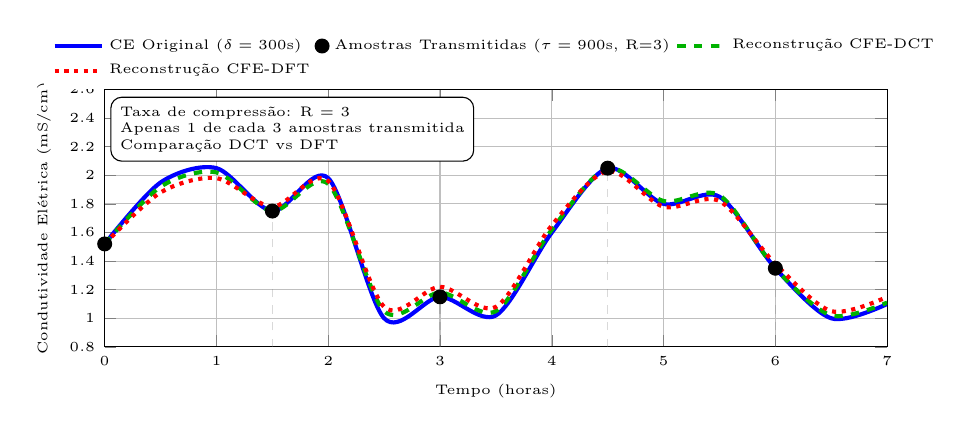
\begin{tikzpicture}
\begin{axis}[
    width=0.95\textwidth,
    height=0.40\textwidth,
    xlabel={Tempo (horas)},
    ylabel={Condutividade Elétrica (mS/cm)},
    grid=major,
    legend style={at={(0.5,-0.15)}, anchor=north, legend columns=2},
    xmin=0, xmax=7,
    ymin=0.8, ymax=2.6,
    xtick={0,1,2,3,4,5,6,7},
    ytick={0.8,1.0,1.2,1.4,1.6,1.8,2.0,2.2,2.4,2.6},
    tick label style={font=\tiny},
    label style={font=\tiny},
    legend style={font=\tiny},
    legend cell align=left,
    legend style={
        at={(0.5,1.)},
        anchor=south,
        legend columns=3,
        font=\tiny,
        draw=none
    },
    % title={Reconstrução da Série Temporal de Condutividade Elétrica (CE)},
    % title style={font=\large\bfseries, yshift=8pt},
]

% CE Original (δ=300s) - Linha azul sólida suave
\addplot[smooth, blue, line width=1.5pt] coordinates {
    (0.0, 1.52) (0.5, 1.95) (1.0, 2.05) (1.5, 1.75) (2.0, 1.98)
    (2.5, 1.00) (3.0, 1.15) (3.5, 1.02) (4.0, 1.60) (4.5, 2.05)
    (5.0, 1.80) (5.5, 1.85) (6.0, 1.35) (6.5, 1.00) (7.0, 1.10)
};
\addlegendentry{CE Original ($\delta=300$s)}

% Amostras Transmitidas (τ=900s, R=3) - Pontos pretos
\addplot[only marks, mark=*, mark size=2.5pt, color=black, fill=black] coordinates {
    (0.0, 1.52) (1.5, 1.75) (3.0, 1.15) (4.5, 2.05) (6.0, 1.35)
};
\addlegendentry{Amostras Transmitidas ($\tau=900$s, R=3)}

% Reconstrução CFE-DCT - Linha verde tracejada suave
\addplot[smooth, green!70!black, dashed, line width=1.5pt] coordinates {
    (0.0, 1.52) (0.5, 1.92) (1.0, 2.02) (1.5, 1.75) (2.0, 1.94)
    (2.5, 1.05) (3.0, 1.18) (3.5, 1.05) (4.0, 1.62) (4.5, 2.05)
    (5.0, 1.82) (5.5, 1.86) (6.0, 1.35) (6.5, 1.02) (7.0, 1.11)
};
\addlegendentry{Reconstrução CFE-DCT}

% Reconstrução CFE-DFT - Linha vermelha pontilhada suave
\addplot[smooth, red, dotted, line width=1.5pt] coordinates {
    (0.0, 1.52) (0.5, 1.88) (1.0, 1.98) (1.5, 1.78) (2.0, 1.96)
    (2.5, 1.08) (3.0, 1.22) (3.5, 1.08) (4.0, 1.65) (4.5, 2.03)
    (5.0, 1.78) (5.5, 1.82) (6.0, 1.38) (6.5, 1.05) (7.0, 1.15)
};
\addlegendentry{Reconstrução CFE-DFT}

% Caixa informativa
\node[draw, fill=white, rounded corners, font=\tiny, align=left, anchor=north west] at (0.05, 2.55) {
    Taxa de compressão: R = 3\\
    Apenas 1 de cada 3 amostras transmitida\\
    Comparação DCT vs DFT
};

% Linha vertical de referência para mostrar os pontos de amostragem
\draw[dashed, gray, opacity=0.3] (1.5,0.8) -- (1.5,1.75);
\draw[dashed, gray, opacity=0.3] (3.0,0.8) -- (3.0,1.15);
\draw[dashed, gray, opacity=0.3] (4.5,0.8) -- (4.5,2.05);
\draw[dashed, gray, opacity=0.3] (6.0,0.8) -- (6.0,1.35);

\end{axis}
\end{tikzpicture}
\caption{Reconstrução qualitativa da série temporal de \gls{ce} comparando métodos CFE-DCT e CFE-DFT. Ambas as reconstruções mantêm a forma do sinal original mesmo transmitindo apenas 33\% das amostras.}
\label{fig:reconstrucao_ce}
\end{figure}